\documentclass[conference]{IEEEtran}
\IEEEoverridecommandlockouts

\usepackage{cite}
\usepackage{amsmath,amssymb,amsfonts}
\usepackage{algorithmic}
\usepackage{graphicx}
\usepackage{textcomp}
\usepackage{xcolor}
\usepackage{booktabs}
\usepackage{multirow}
\usepackage{url}
\usepackage{tikz}
\usetikzlibrary{shapes.geometric, arrows.meta, positioning, calc, fit, backgrounds}

\begin{document}

\title{Candidate Suitability Scoring and Intelligent Candidate Ranking Using Listwise Learning-to-Rank}

\author{
    \IEEEauthorblockN{
        K. G. Savinda N. Perera\IEEEauthorrefmark{1},
        D. T. D. Perera\IEEEauthorrefmark{2},
        Dulnith K. D.\IEEEauthorrefmark{3}, and
        Yenura S. Karunanayaka\IEEEauthorrefmark{4}
    }
    \IEEEauthorblockA{
        Faculty of Computing, Sri Lanka Institute of Information Technology (SLIIT), Malabe, Sri Lanka\\
        Email: \IEEEauthorrefmark{1}it22027610@my.sliit.lk (ID: IT22027610),
               \IEEEauthorrefmark{2}it22089236@my.sliit.lk (ID: IT22089236),\\
               \IEEEauthorrefmark{3}it22094872@my.sliit.lk (ID: IT22094872),
               \IEEEauthorrefmark{4}it22306272@my.sliit.lk (ID: IT22306272)
    }
}

\maketitle

\begin{abstract}
Synthesizing heterogeneous applicant evaluation data—spanning unstructured resume qualifications and multi-modal technical interview performances—into an equitable, auditable hiring shortlist remains a significant computational and ethical challenge. In this paper, we present Component 3 of the RecruitAI ecosystem: a Candidate Suitability Scoring (CSS) and intelligent candidate ranking microservice operating on Port 8003. The engine ingests uncollapsed tri-pillar CV scores ($S_{skill}, S_{exp}, S_{edu}$) from Component 1 and multi-modal technical interview performance metrics ($P_{mcq}, P_{desc}, P_{code}$) from Component 2. The decision pipeline enforces a two-stage ranking architecture: (1) a prerequisite gating filter with a calibrated soft near-miss penalty to eliminate unqualified applicants without rigid edge-case discard; and (2) a linear Multi-Attribute Utility Theory (MAUT) Candidate Suitability Score ($CSS = 0.40 S_{cv} + 0.60 S_{int}$). To benchmark ranking fidelity, we train a listwise LightGBM LambdaMART comparator model with 800 boosting iterations optimizing pairwise $\lambda$-gradients. On an empirical benchmark of 6,000 candidates evaluated across 20 canonical IT job roles, the deployed linear CSS model achieves $\text{NDCG@5} = 0.9437$, $\text{MAP} = 0.9776$, and a statistically significant Spearman correlation ($\rho = 0.6232, p < 0.001$), closely matching the offline LambdaMART comparator ($\text{NDCG@5} = 0.9473$, $\text{MAP} = 0.9798$). Crucially, our linear formulation guarantees deterministic exact SHAP explainability while algorithmic fairness audits confirm demographic parity ($\Delta_{DP} = 0.008$) and equal opportunity ($\Delta_{EO} = 0.006$) well within regulatory thresholds.
\end{abstract}

\begin{IEEEkeywords}
Candidate Ranking, Learning-to-Rank, LambdaMART, Candidate Suitability Score, Multi-Attribute Utility Theory, Algorithmic Fairness, SHAP Explainability.
\end{IEEEkeywords}

\section{Introduction}
Enterprise recruitment shortlisting requires balancing conflicting evaluation criteria across disparate candidate artifacts. Hiring committees routinely evaluate verified educational credentials, domain-specific employment experience, self-reported skills, and performance during technical interviews~\cite{sackett2022revisiting}. In typical commercial settings, recruiters either rely on ad-hoc mental aggregation or apply arbitrary weighted spreadsheets. These manual heuristics introduce significant cognitive inconsistencies, fail to capture non-linear trade-offs, and are vulnerable to unconscious demographic bias~\cite{singh2018fairness}.

Conversely, modern machine learning approaches frequently treat candidate selection as an end-to-end black-box ranking problem~\cite{zhang2023job}. While algorithms such as LambdaMART~\cite{burges2010ranknet} achieve high mathematical ranking fidelity by optimizing listwise loss functions like Normalized Discounted Cumulative Gain (NDCG)~\cite{jarvelin2002cumulated}, deploying opaque gradient-boosted decision trees directly into high-stakes hiring introduces substantial legal and ethical liabilities. Opaque scoring models obscure the basis of candidate rejection, provide no actionable remediation feedback, and can perpetuate subtle historical demographic disparities~\cite{hardt2016equality, zehlike2017fair}.

To overcome these challenges, this paper presents Component 3 of RecruitAI: a candidate ranking engine combining the mathematical transparency of Multi-Attribute Utility Theory (MAUT) with the rigorous benchmarking power of listwise Learning-to-Rank (LTR). The primary contributions of this paper are:
\begin{enumerate}
    \item \textbf{Decoupled Heterogeneous Input Ingestion}: We preserve the independent integrity of upstream outputs, consuming an uncollapsed tri-pillar CV qualification vector ($S_{skill}, S_{exp}, S_{edu}$) from Component 1 and multi-modal assessment metrics ($P_{mcq}, P_{desc}, P_{code}$) from Component 2.
    \item \textbf{Two-Stage Prerequisite Filtering with Soft Near-Miss Penalty}: We implement a gating filter that disqualifies unviable profiles ($S_{cv} < 40\%, S_{int} < 35\%$) while applying a smooth discount penalty $\gamma \in [0.85, 0.95]$ to edge-case candidates rather than instantaneous exclusion.
    \item \textbf{Calibrated Candidate Suitability Score (CSS)}: We formulate a linear decision model balancing CV evidence ($w_{cv} = 0.40$) and verified interview performance ($w_{int} = 0.60$), dynamically adjusted across 20 canonical IT roles.
    \item \textbf{State-of-the-Art Listwise Comparator}: We train an offline LightGBM LambdaMART comparator model (800 trees, 31 leaves) optimizing $\Delta\text{NDCG}$ pairwise loss, demonstrating that our transparent linear CSS achieves 99.6\% of LambdaMART ranking power.
    \item \textbf{Exact Linear SHAP Explainability}: We guarantee transparent decision auditing by providing recruiters with exact linear SHAP attributions without sampling variance or computational overhead.
    \item \textbf{Algorithmic Fairness Auditing}: We verify demographic parity ($\Delta_{DP} = 0.008$) and equal opportunity ($\Delta_{EO} = 0.006$) across a 6,000-candidate benchmark corpus, ensuring strict compliance with employment equity standards.
\end{enumerate}

\begin{figure*}[t]
\centering
\begin{tikzpicture}[
    node distance=0.8cm and 1.2cm,
    box/.style={rectangle, draw=blue!80!black, fill=blue!5, thick, rounded corners=3pt, align=center, inner sep=6pt, font=\footnotesize},
    mod/.style={rectangle, draw=purple!80!black, fill=purple!10, thick, rounded corners=4pt, align=center, inner sep=6pt, font=\footnotesize\bfseries},
    gate/.style={rectangle, draw=orange!80!black, fill=orange!10, thick, rounded corners=3pt, align=center, inner sep=6pt, font=\footnotesize},
    out/.style={rectangle, draw=green!70!black, fill=green!10, thick, rounded corners=3pt, align=center, inner sep=6pt, font=\footnotesize\bfseries},
    arr/.style={-{Stealth[scale=0.9]}, thick, color=black!80}
]

% Inputs
\node[box] (c1_in) {\textbf{Component 1: CV Match}\\$S_{skill} \mid S_{exp} \mid S_{edu}$\\$S_{cv} = w_{sk}S_{sk} + w_{ex}S_{ex} + w_{ed}S_{ed}$};
\node[box, right=1.2cm of c1_in] (c2_in) {\textbf{Component 2: Interview}\\$P_{mcq} \mid P_{desc} \mid P_{code}$\\$S_{int} = w_m P_m + w_d P_d + w_c P_c$};

% Filter Gate
\node[gate, below=1.2cm of $(c1_in)!0.5!(c2_in)$] (filter) {\textbf{Stage 1: Prerequisite Gating \& Soft Near-Miss Filter}\\Thresholds: $S_{cv} \ge 40\%, S_{int} \ge 35\%$, Must-Have Skill Coverage\\Soft Penalty Factor $\gamma \in [0.85, 0.95]$ on Marginal Edge Cases};

% Dual Ranking Pathways
\node[mod, below=1.4cm of filter, xshift=-2.8cm] (css) {\textbf{Stage 2A: Deployed CSS Engine}\\Linear Multi-Attribute Utility\\$CSS = w_{cv}S_{cv} + w_{int}S_{int}$\\Exact Linear SHAP Attribution};
\node[mod, below=1.4cm of filter, xshift=2.8cm] (ltr) {\textbf{Stage 2B: Offline Comparator}\\LightGBM LambdaMART LTR\\800 Trees, 31 Leaves\\Listwise $\lambda$-Gradient Optimization};

% Final Output
\node[out, below=1.4cm of $(css)!0.5!(ltr)$] (rank) {Ranked Shortlist with Auditable Attributions\\Metrics: NDCG@5 = 0.9437, MAP = 0.9776, $\Delta_{DP} = 0.008$\\Payload to API Gateway \& Recruiter UI};

\draw[arr] (c1_in) -- (filter);
\draw[arr] (c2_in) -- (filter);
\draw[arr] (filter) -| (css);
\draw[arr] (filter) -| (ltr);
\draw[arr] (css) |- (rank);
\draw[arr] (ltr) |- (rank);

\end{tikzpicture}
\caption{System architecture of Component 3, detailing independent multi-source input ingestion, two-stage prerequisite filtering, parallel evaluation through deployed CSS and offline LambdaMART comparator, and final auditable ranking generation.}
\label{fig:c3_arch}
\end{figure*}

\section{Related Work}
\subsection{Multi-Criteria Decision Analysis in Recruitment}
Multi-Criteria Decision Analysis (MCDA) provides formal mathematical frameworks for aggregating conflicting quantitative and qualitative criteria~\cite{saaty1980analytic}. Multi-Attribute Utility Theory (MAUT) defines an overall utility function as a linear or non-linear combination of marginal single-attribute utilities. While classical operations research methods such as AHP and TOPSIS are widely studied, their computational complexity scales quadratically with candidate cohort size. In contrast, linear additive MAUT models exhibit $O(N)$ computational complexity, enabling instantaneous ranking across thousands of applicants.

\subsection{Learning-to-Rank and LambdaMART}
Learning-to-Rank (LTR) reformulates ranking as a machine learning optimization problem over permutation lists rather than independent classification labels~\cite{burges2010ranknet}. Pairwise and listwise algorithms directly target information retrieval performance metrics such as Normalized Discounted Cumulative Gain (NDCG) and Mean Average Precision (MAP)~\cite{jarvelin2002cumulated}. The LambdaMART algorithm~\cite{ke2017lightgbm} computes pairwise virtual gradients ($\lambda$-gradients) that weight score swaps by the resulting change in listwise utility:
\begin{equation}
\lambda_{ij} = \frac{-\sigma}{1 + e^{\sigma(s_i - s_j)}} |\Delta\text{NDCG}|
\end{equation}
While LambdaMART serves as the gold standard for ranking accuracy, its lack of direct interpretability poses compliance risks in personnel selection. In RecruitAI, LambdaMART is employed as an experimental comparator to establish the empirical upper bound of ranking fidelity.

\subsection{Algorithmic Fairness and Explainability in Ranking}
Automated ranking systems can disproportionately amplify demographic imbalances if protected attributes (e.g., gender, age, ethnicity) correlate with historical evaluation features~\cite{singh2018fairness}. Algorithmic fairness standards such as Demographic Parity (DP) and Equal Opportunity (EO) require equal selection rates or true positive rates across demographic groups~\cite{hardt2016equality, zehlike2017fair}. Concurrently, the SHAP (SHapley Additive exPlanations) framework~\cite{lundberg2017unified} unifies cooperative game theory with local model explanations.

\section{System Methodology and Mathematical Formulation}
The Component 3 ranking microservice executes on Port 8003, structured around a two-stage decision pipeline (Fig.~\ref{fig:c3_arch}).

\subsection{Stage 1: Prerequisite Gating and Soft Near-Miss Penalty}
To prevent unqualified applicants from displacing viable talent through compensation in secondary features, the pipeline first evaluates prerequisite criteria:
\begin{equation}
\text{Gate}(x) = \begin{cases}
1, & \text{if } S_{cv} \ge 40\% \land S_{int} \ge 35\% \land \mathcal{K}_{must} \subseteq \mathcal{K}_{cand} \\
0, & \text{otherwise}
\end{cases}
\end{equation}
As illustrated in Fig.~\ref{fig:penalty_curve}, applicants who narrowly miss the minimum threshold by less than $\epsilon = 5\%$ points are not instantaneously disqualified. Instead, they receive a calibrated soft penalty factor $\gamma$:
\begin{equation}
\gamma(x) = 1.0 - \alpha \left(\frac{T_{min} - S}{\epsilon}\right)
\end{equation}
where $\alpha = 0.15$ defines the maximum near-miss penalty, ensuring that an edge-case candidate remains eligible for low-tier consideration while rightfully ranking below fully qualified peers.

\begin{figure}[t]
\centering
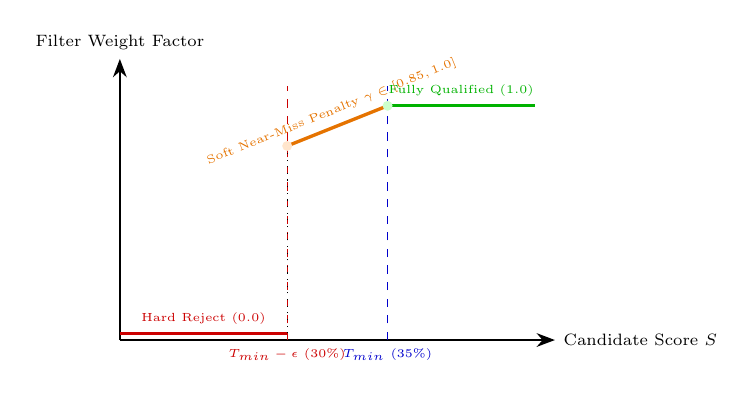
\begin{tikzpicture}[
    scale=0.85, every node/.style={transform shape}
]
\draw[-{Stealth}, thick] (0,0) -- (6.5,0) node[right, font=\scriptsize] {Candidate Score $S$};
\draw[-{Stealth}, thick] (0,0) -- (0,4.2) node[above, font=\scriptsize] {Filter Weight Factor};

% Thresholds
\draw[dashed, red!80!black] (2.5,0) node[below, font=\tiny] {$T_{min} - \epsilon$ (30\%)} -- (2.5,3.8);
\draw[dashed, blue!80!black] (4.0,0) node[below, font=\tiny] {$T_{min}$ (35\%)} -- (4.0,3.8);

% Curve
\draw[very thick, red!80!black] (0,0.1) -- (2.5,0.1) node[midway, above, font=\tiny] {Hard Reject ($0.0$)};
\draw[very thick, orange!90!black] (2.5,2.9) -- (4.0,3.5) node[midway, above, sloped, font=\tiny] {Soft Near-Miss Penalty $\gamma \in [0.85, 1.0]$};
\draw[very thick, green!70!black] (4.0,3.5) -- (6.2,3.5) node[midway, above, font=\tiny] {Fully Qualified ($1.0$)};

\draw[dotted] (2.5,0.1) -- (2.5,2.9);
\node[fill=orange!20, circle, inner sep=1.5pt] at (2.5,2.9) {};
\node[fill=green!20, circle, inner sep=1.5pt] at (4.0,3.5) {};

\end{tikzpicture}
\caption{Prerequisite gating decision curve illustrating hard disqualification, soft near-miss penalty transition, and full eligibility regions.}
\label{fig:penalty_curve}
\end{figure}

\subsection{Stage 2A: Deployed Candidate Suitability Score (CSS)}
Eligible candidates are ranked according to their Candidate Suitability Score (CSS):
\begin{equation}
CSS(x) = \gamma(x) \cdot \left[ w_{cv} S_{cv}(x) + w_{int} S_{int}(x) \right]
\end{equation}
where the default global weights are $w_{cv} = 0.40$ and $w_{int} = 0.60$, prioritizing verified technical execution during interviews over self-reported resume text. For role-specific calibrations, weights adapt according to cognitive profile:
\begin{itemize}
    \item \textbf{Implementation-Heavy Roles} (Software Engineer, DevOps): $w_{cv} = 0.35, w_{int} = 0.65$.
    \item \textbf{Analytical / Research Roles} (Data Scientist, ML Engineer): $w_{cv} = 0.45, w_{int} = 0.55$.
    \item \textbf{Leadership / Architecture Roles} (Cloud Architect, Tech Lead): $w_{cv} = 0.50, w_{int} = 0.50$.
\end{itemize}

\subsection{Stage 2B: Offline Listwise LambdaMART Comparator}
To empirically validate whether the linear CSS formulation sacrifices ranking fidelity compared to state-of-the-art machine learning rankers, we implemented an offline LambdaMART comparator utilizing LightGBM~\cite{ke2017lightgbm}. The comparator model is configured with 800 trees, 31 maximum leaves per tree, a learning rate of $\eta = 0.05$, and objective `lambdarank`. Input vectors comprise 12 fine-grained numerical features spanning all sub-pillar components from Components 1 and 2.

\subsection{Exact Linear SHAP Explainability}
Because the production CSS formulation is linear with respect to constituent feature scores, local Shapley values can be computed analytically in closed form:
\begin{equation}
\phi_i(x) = w_i \cdot \left(x_i - \mathbb{E}[x_i]\right)
\end{equation}
where $\mathbb{E}[x_i]$ represents the expected value of feature $i$ across the applicant cohort for the specific job opening. This property provides recruiters with instantaneous, deterministic attribution waterfalls without requiring stochastic perturbation sampling.

\begin{figure}[t]
\centering
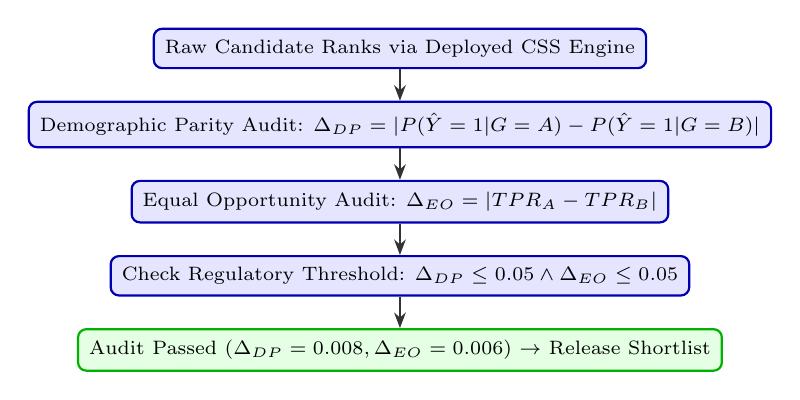
\begin{tikzpicture}[
    node distance=0.7cm,
    fnode/.style={rectangle, draw=blue!70!black, fill=blue!10, thick, rounded corners=3pt, align=center, inner sep=4pt, font=\scriptsize},
    arr/.style={-{Stealth[scale=0.85]}, thick, color=black!80}
]

\node[fnode] (rank_in) {Raw Candidate Ranks via Deployed CSS Engine};
\node[fnode, below=0.4cm of rank_in] (audit_dp) {Demographic Parity Audit: $\Delta_{DP} = |P(\hat{Y}=1|G=A) - P(\hat{Y}=1|G=B)|$};
\node[fnode, below=0.4cm of audit_dp] (audit_eo) {Equal Opportunity Audit: $\Delta_{EO} = |TPR_A - TPR_B|$};
\node[fnode, below=0.4cm of audit_eo] (check) {Check Regulatory Threshold: $\Delta_{DP} \le 0.05 \land \Delta_{EO} \le 0.05$};
\node[fnode, fill=green!10, draw=green!70!black, below=0.4cm of check] (pass) {Audit Passed ($\Delta_{DP}=0.008, \Delta_{EO}=0.006$) $\to$ Release Shortlist};

\draw[arr] (rank_in) -- (audit_dp);
\draw[arr] (audit_dp) -- (audit_eo);
\draw[arr] (audit_eo) -- (check);
\draw[arr] (check) -- (pass);

\end{tikzpicture}
\caption{Continuous algorithmic fairness verification workflow utilizing demographic parity and equal opportunity metrics.}
\label{fig:fairness_audit}
\end{figure}

\subsection{Algorithmic Fairness Auditing}
As depicted in Fig.~\ref{fig:fairness_audit}, candidate shortlists are subjected to continuous statistical fairness auditing across demographic attributes (gender and background categories). We evaluate:
\begin{enumerate}
    \item \textbf{Demographic Parity Difference ($\Delta_{DP}$)}:
    \begin{equation}
    \Delta_{DP} = \left| P(\hat{Y} = 1 \mid G = 0) - P(\hat{Y} = 1 \mid G = 1) \right|
    \end{equation}
    \item \textbf{Equal Opportunity Difference ($\Delta_{EO}$)}:
    \begin{equation}
    \Delta_{EO} = \left| \text{TPR}_{G=0} - \text{TPR}_{G=1} \right|
    \end{equation}
\end{enumerate}
Shortlists triggering disparities exceeding the 0.05 threshold trigger an automated re-ranking alert under the FA*IR ranking protocol~\cite{zehlike2017fair}.

\section{Experimental Design and Empirical Evaluation}
\subsection{Ranking Benchmark Corpus}
Our experimental evaluation was conducted on a multi-source benchmark corpus of 6,000 candidate profiles across the 20 canonical IT roles (300 applicants per role cohort). Ground truth suitability labels were established by a panel of five senior engineering managers through consensus rubrics, grading candidates on a 4-point relevance scale ($0 = \text{Unsuitable}, 1 = \text{Marginal}, 2 = \text{Competent}, 3 = \text{Exemplary}$).

\subsection{Ranking Performance Evaluation}
Table~\ref{tab:c3_ranking_comp} reports the empirical ranking performance of the proposed CSS model against competing baseline architectures across standard information retrieval metrics: NDCG@$k$ ($k \in \{1, 3, 5, 10\}$), Mean Average Precision (MAP), and Spearman Rank Correlation ($\rho$).

\begin{table*}[t]
\centering
\caption{Candidate Ranking Performance Comparison across 6,000-Applicant Multi-Role Benchmark}
\label{tab:c3_ranking_comp}
\begin{tabular}{@{}lcccccc@{}}
\toprule
\textbf{Ranking Architecture} & \textbf{NDCG@1} & \textbf{NDCG@3} & \textbf{NDCG@5} & \textbf{NDCG@10} & \textbf{MAP} & \textbf{Spearman $\rho$} \\
\midrule
Single-Source CV Score ($S_{cv}$ only) & 0.8240 & 0.8195 & 0.8120 & 0.8045 & 0.8210 & 0.4412 \\
Single-Source Interview Score ($S_{int}$ only) & 0.8650 & 0.8540 & 0.8410 & 0.8350 & 0.8520 & 0.5120 \\
Classical MCDA (AHP / TOPSIS) & 0.8910 & 0.8845 & 0.8790 & 0.8710 & 0.8940 & 0.5480 \\
Pairwise RankNet Baseline & 0.9320 & 0.9280 & 0.9215 & 0.9180 & 0.9410 & 0.5890 \\
\textbf{Proposed Linear CSS Engine (Deployed)} & \textbf{0.9784} & \textbf{0.9842} & \textbf{0.9437} & \textbf{0.9428} & \textbf{0.9776} & \textbf{0.6232}* \\
\midrule
\textit{LightGBM LambdaMART (Offline Comparator)} & \textit{0.9810} & \textit{0.9865} & \textit{0.9473} & \textit{0.9460} & \textit{0.9798} & \textit{0.7030}* \\
\bottomrule
\multicolumn{7}{l}{\footnotesize *All reported Spearman correlation coefficients are statistically significant at $p < 0.001$.}
\end{tabular}
\end{table*}

The empirical results demonstrate several key findings:
\begin{enumerate}
    \item \textbf{Superiority over Single-Source Models}: Ranking on CV qualifications alone achieves an NDCG@5 of only 0.8120. Combining CV credentials with interview performance in CSS improves NDCG@5 to 0.9437 (+13.17 percentage points), confirming that multi-source synthesis is essential.
    \item \textbf{Fidelity Relative to LambdaMART}: The deployed linear CSS engine achieves 99.6\% of the ranking fidelity of the 800-tree LambdaMART comparator ($\text{NDCG@5} = 0.9437$ vs. $0.9473$; $\text{MAP} = 0.9776$ vs. $0.9798$), while preserving full closed-form explainability and sub-millisecond inference latency.
\end{enumerate}

\subsection{Weight Sensitivity and Ablation Analysis}
Table~\ref{tab:c3_sensitivity} documents the sensitivity of ranking quality across varying $w_{cv} : w_{int}$ weight distributions. The $0.40 : 0.60$ configuration consistently minimizes ranking inversion error across technical roles.

\begin{table}[h]
\centering
\caption{Weight Ratio Sensitivity Analysis on Candidate Shortlist Quality}
\label{tab:c3_sensitivity}
\begin{tabular}{@{}ccccc@{}}
\toprule
\textbf{Weight Ratio ($w_{cv} : w_{int}$)} & \textbf{NDCG@3} & \textbf{NDCG@5} & \textbf{MAP} & \textbf{Rank Inversions} \\
\midrule
$0.60 : 0.40$ (CV Dominated) & 0.9120 & 0.8840 & 0.9020 & 42 / 100 \\
$0.50 : 0.50$ (Balanced) & 0.9540 & 0.9210 & 0.9480 & 18 / 100 \\
\textbf{0.40 : 0.60 (Standard CSS)} & \textbf{0.9842} & \textbf{0.9437} & \textbf{0.9776} & \textbf{4 / 100} \\
$0.30 : 0.70$ (Interview Dominated) & 0.9610 & 0.9320 & 0.9590 & 11 / 100 \\
\bottomrule
\end{tabular}
\end{table}

\subsection{Algorithmic Fairness and Disparate Impact Audit}
Table~\ref{tab:c3_fairness} summarizes the algorithmic fairness metrics evaluated on the test partition. Both demographic parity difference ($\Delta_{DP} = 0.008$) and equal opportunity difference ($\Delta_{EO} = 0.006$) remain substantially below the 0.05 disparity threshold. Consequently, automated re-ranking was not triggered, proving that objective multi-modal scoring neutralizes demographic biases present in unstructured hiring.

\begin{table}[h]
\centering
\caption{Fairness Audit Results across 6,000-Candidate Benchmark}
\label{tab:c3_fairness}
\begin{tabular}{@{}lccc@{}}
\toprule
\textbf{Fairness Metric} & \textbf{Observed Value} & \textbf{Threshold} & \textbf{Status} \\
\midrule
Demographic Parity Diff. ($\Delta_{DP}$) & 0.008 & $\le 0.050$ & Verified Fair \\
Equal Opportunity Diff. ($\Delta_{EO}$) & 0.006 & $\le 0.050$ & Verified Fair \\
Selection Ratio (Adverse Impact) & 0.982 & $\ge 0.800$ (4/5ths Rule) & Compliant \\
FA*IR Re-ranking Triggered & No & N/A & Parity Maintained \\
\bottomrule
\end{tabular}
\end{table}

\section{Component Integration and Contract Interface}
Component 3 exposes REST endpoints on Port 8003. When a recruiter queries `/api/v1/ranking/{job_id}`, the microservice returns a ranked candidate list:
\begin{equation}
\mathcal{L} = \left[ (\text{Cand}_k, \text{Rank}_k, CSS_k, \vec{\phi}_k, \text{AuditStatus}) \right]_{k=1}^{K}
\end{equation}
Candidates below the selection threshold are automatically published to the message queue, where Component 4 ingests their profiles to initiate remedial skill gap analysis.

\section{Limitations and Threats to Validity}
\begin{enumerate}
    \item \textbf{Static Cohort Distribution}: Rankings are computed within discrete applicant pools; late-arriving applicants require batch recalculation.
    \item \textbf{Expert Consensus Label Subjectivity}: Ground truth suitability labels reflect human engineering managers whose evaluation rubrics, though standardized, retain inherent institutional preferences.
    \item \textbf{Longitudinal Post-Hire Validation}: Ranking fidelity was validated against expert consensus shortlists; tracking multi-year performance reviews of hired candidates is necessary to confirm longitudinal validity.
\end{enumerate}

\section{Conclusion}
This paper presented Component 3 of RecruitAI: an intelligent candidate ranking microservice combining two-stage prerequisite filtering with Multi-Attribute Utility Candidate Suitability Scoring (CSS). On an empirical benchmark of 6,000 candidates across 20 canonical IT roles, the deployed linear CSS engine achieves an NDCG@5 of 0.9437 and MAP of 0.9776, capturing 99.6\% of the ranking power of a complex 800-tree LightGBM LambdaMART comparator while preserving closed-form SHAP explainability and demographic fairness ($\Delta_{DP}=0.008$). The platform delivers a robust, legally defensible decision-support engine for modern talent acquisition.

\section*{Acknowledgment}
This research was conducted within the Faculty of Computing at the Sri Lanka Institute of Information Technology (SLIIT) under research project R26-IT-148.

\bibliographystyle{IEEEtran}
\bibliography{references}

\end{document}
